\chapter{Advanced Debug Unit}

The advanced debug unit has an AXI master interface to access peripherals and
memories. In contrast to PulpinoV1 the adv. debug unit does no longer feature
 a specialized debug interface to readout all core registers.

All core registers are now memory mapped which means that they can be read over
 the AXI interface. Hence, debugging is not only possible over JTAG, but also SPI
 or any other interface.

The JTAG signals are connected to pins of the SoC.

\begin{figure}[H]
  \centering
  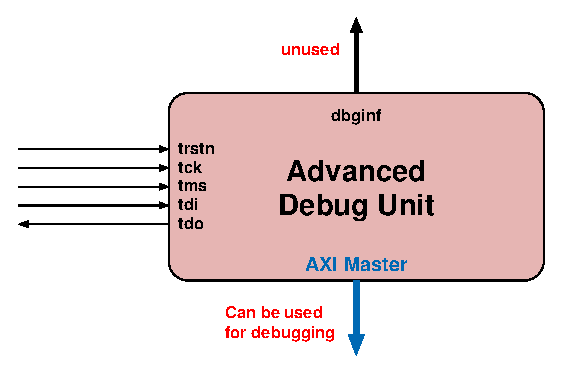
\includegraphics[width=0.5\textwidth]{./figures/adv_dbg_unit}
  \caption{Advanced Debug Unit.}
  \label{fig:adv_dbg_unit}
\end{figure}

For more details please take a look at the documentation of the advanced debug unit.


